% -*- TeX-master: "main" -*-

\section{Package syntax and semantics}
\label{sec:syntax}
This section contains a definition of the syntax and semantics of the Spatial package for \sbmlthreecore.  The Spatial package involves several new object classes, and extends the existing \Model, \Compartment, \Species, \Reaction, and \Parameter object class.  \sec{examples} contains complete examples of using the constructs in SBML models.

{\color{red} Lucian: \notice Periodically when I have comments, I'll put them in sections that look like this--in red, with the pointy-hand icon off to the side.  They tend to be design questions I had when creating this document for parts I thought were not clear, or are suggestions for changes that could be made.}


\subsection{Overview of spatial extension}
The SBML \Compartment, \Reaction and \Species, and molecular transport mechanisms (\DiffusionCoefficient, \AdvectionCoefficient, \BoundaryCondition) are mapped to geometric domains to describe spatial models within SBML.  The primary mechanism to accomplish this mapping is to simply map \Compartments to collections of geometric Domains called \DomainTypes.  Each \Domain is a contiguous patch of volumetric space or a contiguous surface patch that is ultimately described by a single system of equations (whichever mathematical framework is used).  In analogy with initial conditions, the mathematical system defined within a domain often needs a definition of what happens at the domain boundary (e.g. boundary conditions) to complete the specification.  Because of this, the boundaries between adjacent domains need to be identified so that appropriate boundary conditions can be specified.  For compactness of representation, rather than map to each individual \Domain, \Compartments are mapped to \DomainTypes, along with the corresponding \Species and \Reactions (with the new compartment attribute).

\subsubsection{Geometry}
The \Geometry object within a model is completely modular and does not reference the rest of the model, promoting reuse of the same geometry in different models.  The geometry separately defines a coordinate system, a list of domain types, a list of domains and their adjacency relationships, and a list of alternate geometric representations.

\subsubsection{Alternative \GeometryDefinitions}
Modeling and simulation tools will each natively support some subset (often just one) of the possible \GeometryDefinitions (analytic, sampled field, constructive solid geometry, and parametric shapes ).  Interoperability will be enhanced if tools write as many geometry definitions as they are able.  Upon reading the model, a tool will typically choose the most convenient geometry definition, i.e. the one that it natively supports.  If a tool does not edit the geometry, it has the ability to preserve the alternate representations during model editing (because the mapping of the model to the geometry is not stored in the geometry).

There are two general classes of geometric representation specification: those that explicitly specify surfaces and those that implicitly specify surfaces.  For example, a level set is a field where a specific isosurface of the field specifies a geometric surface.  A geometry described using constructive solid geometry of geometric primitives (e.g. spheres, cylinders) specifies directly which points are "inside" an object.  Alternatively, explicit surface representations explicitly declare the set of points belonging to surfaces (e.g. polygonal tessellations).



% --------------------------------------------------------------------------
\subsection{Namespace URI and other declarations necessary for using this package}
\label{xml-namespace}
Every SBML Level~3 package is identified uniquely by an XML namespace URI.  For an SBML document to be able to use a given Level~3 package, it must declare the use of that package by referencing its URI.  The following is the namespace URI for this version of the Spatial package for \sbmlthreecore:
\begin{center}
\uri{http://www.sbml.org/sbml/level3/version1/spatial/version1}
\end{center}

In addition, SBML documents using a given package must indicate whether the package can be used to change the mathematical interpretation of a model.  This is done using the attribute \token{required} on the \token{<sbml>} element in the SBML document.  For the Spatial package, the value of this attribute must be \val{true}, because the use of the Spatial package can change the mathematical meaning of a model.

The following fragment illustrates the beginning of a typical SBML model using \sbmlthreecore and this version of the Spatial package:

\begin{example}
<?xml version="1.0" encoding="UTF-8"?>
<sbml xmlns="http://www.sbml.org/sbml/level3/version1/core" level="3" version="1"
      xmlns:spatial="http://www.sbml.org/sbml/level3/version1/spatial/version1"
      spatial:required="true">
\end{example}


\subsection{Primitive data types}
\label{new-primitive-types}

The Spatial package uses a number of the primitive data types described in Section~3.1 of the \sbmlthreecore specification, and adds several additional primitive types described below.


\subsubsection{Type \fixttspace\primtypeNC{SpId}}
\label{primtype-spid}

The type \primtype{SpId} is derived from \primtype{SId}
(\sbmlthreecore specification Section~3.1.7) and has identical syntax. The \primtype{SpId} type is used as the data type for the identifiers of various objects in the Spatial Processes package.  The purpose of having a separate type for such identifiers is to enable the space of possible spatial identifier values to be separated from the space of all other identifier values in SBML.  The equality of \primtype{SpId} values is determined by an exact character sequence match; i.e., comparisons of these identifiers must be performed in a case-sensitive manner.


\subsubsection{Type \fixttspace\primtypeNC{SpIdRef}}
\label{primtype-spidref}

Type \primtype{SpIdRef} is used for all attributes that refer to identifiers of type \primtype{SpId}.  This type is derived from \primtype{SpId}, but with the restriction that the value of an attribute having type \primtype{SpIdRef} must match the value of a \primtype{SpId} attribute in the relevant model;  in other words, the value of the attribute must be an existing spatial identifier in the referenced model.  As with \primtype{SpId}, the equality of \primtype{SpIdRef} values is determined by exact character sequence match; i.e., comparisons of these identifiers must be performed in a case-sensitive manner.


\subsubsection{Type \fixttspace\primtypeNC{BoundaryConditionKind}}
\label{primtype-boundaryconditionkind}

The \primtype{BoundaryConditionKind} primitive data type is used in the definition of the \BoundaryCondition class.  The type \primtype{BoundaryConditionKind} is derived from type \primtype{string} and its values are restricted to being one of the following possibilities: \val{Robin\_valueCoefficient}, \val{Robin\_inwardNormalGradientCoefficient}, \val{Robin\_sum}, \val{\changed{Neumann}}, and \val{\changed{Dirichlet}}.  Attributes of type \primtype{BoundaryConditionKind} cannot take on any other values.  The meaning of these values is discussed in the context of the \BoundaryCondition class's definition in \sec{BoundaryCondition-class}.


\subsubsection{Type \fixttspace\primtypeNC{\changed{CoordinateKind}}}
\label{primtype-componentkind}

The \primtype{\changed{CoordinateKind}} primitive data type is used in the definition of the \CoordinateComponent class.  \primtype{\changed{CoordinateKind}} is derived from type \primtype{string} and its values are restricted to being one of the following possibilities: \val{cartesianX}, \val{cartesianY}, and \val{cartesianZ}.
%, \val{spherical\-Radius}, \val{sphericalAzimuth}, \val{sphericalElevation}, \val{cylindrical\-Radius}, \val{cylindricalAzimuth}, \val{cylindricalHeight}, \val{polarRadius}, and \val{polarAzimuth}.
Attributes of type \primtype{\changed{CoordinateKind}} cannot take on any other values.  The meaning of these values is discussed in the context of the \CoordinateComponent class's definition in \sec{CoordinateComponent-class}.

Other \primtype{\changed{CoordinateKind}} types are held in reserve for future versions of this specification, and may include \val{spherical\-Radius}, \val{sphericalAzimuth}, \val{sphericalElevation}, \val{cylindrical\-Radius}, \val{cylindricalAzimuth}, \val{cylin\-dricalHeight}, \val{polarRadius}, and \val{polarAzimuth}.



%\subsubsection{Type \fixttspace\primtypeNC{CoordinateKind}}
%\label{primtype-coordinatekind}
%
%The \primtype{CoordinateKind} primitive data type is used in the definition of the \CoordinateComponent class.  The type \primtype{CoordinateKind} is derived from type \primtype{string} and its values are restricted to being one of the following possibilities: \val{normal}, \val{symmetrical}, and \val{fixed}.  Attributes of type \primtype{CoordinateKind} cannot take on any other values.  The meaning of these values is discussed in the context of the \CoordinateComponent class's definition in \sec{CoordinateComponent-class}.


\subsubsection{Type \fixttspace\primtypeNC{DiffusionKind}}
\label{primtype-diffusionkind}

The \primtype{DiffusionKind} primitive data type is used in the definition of the \DiffusionCoefficient class.  \primtype{DiffusionKind} is derived from type \primtype{string} and its values are restricted to being one of the following possibilities: \val{isotropic}, \changed{\val{anisotropic}}, and \val{tensor}.  Attributes of type \primtype{DiffusionKind} cannot take on any other values.  The meaning of these two values is discussed in the context of the \DiffusionCoefficient class's definition in \sec{DiffusionCoefficient-class}.


\subsubsection{Type \fixttspace\primtypeNC{FunctionKind}}
\label{primtype-functionkind}

The \primtype{FunctionKind} primitive data type is used in the definition of the \AnalyticVolume class.  The type \primtype{FunctionKind} is derived from type \primtype{string} and its values are restricted to being one of the \changed{single} possibility \val{layered}.  Attributes of type \primtype{FunctionKind} cannot take on any other values.  The meaning of these values is discussed in the context of the \AnalyticVolume class's definition in \sec{AnalyticVolume-class}.


\subsubsection{Type \fixttspace\primtypeNC{GeometryKind}}
\label{primtype-geometrykind}

The \primtype{GeometryKind} primitive data type is used in the definition of the \Geometry class.  \primtype{GeometryKind} is derived from type \primtype{string} and its values are restricted to being the single possibility \val{cartesian}.  Other \primtype{GeometryKind} types are held in reserve for future versions of this specification, and may include \val{cylindrical}, \val{spherical}, and \val{polar}.  Attributes of type \primtype{GeometryKind} cannot take on any other values.  The meaning of these values is discussed in the context of the \Geometry class's definition in \sec{Geometry-class}.


\subsubsection{Type \fixttspace\primtypeNC{SetOperation}}
\label{primtype-setoperation}

The \primtype{SetOperation} primitive data type is used in the definition of the \CSGSetOperator class.  The type \primtype{SetOperation} is derived from type \primtype{string} and its values are restricted to being one of the following possibilities: \val{union}, \val{intersection}, and \val{difference}.  Attributes of type \primtype{SetOperation} cannot take on any other values.  The meaning of these values is discussed in the context of the \CSGSetOperator class's definition in \sec{CSGSetOperator-class}.


\subsubsection{Type \fixttspace\primtypeNC{doubleArray}}
\label{primtype-doublearray}

The \primtype{doubleArray} primitive data type is a space-delimited list of \primtype{double} values in a single string.  


\subsubsection{Type \fixttspace\primtypeNC{integerArray}}
\label{primtype-integerarray}

The \primtype{integerArray} primitive data type is a space-delimited list of \primtype{integer} values in a single string.  

\clearpage


\subsection{The extended \Model object}
\label{extended-model-class}
The \Model object is extended in the spatial package to contain a new \Geometry child, as seen in
\fig{model-uml}. The \Geometry element is contained in the Model element in the 'spatial' namespace. In order to specify a spatial geometry, some of the existing SBML elements need to be extended (\Compartment, \Species, \Parameter, and \Reaction). These extensions to the SBML elements are discussed in the sections that follow.
 
\begin{figure}[ht]
  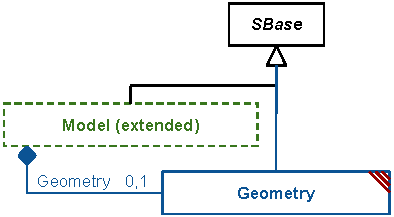
\includegraphics{figs/extended-model-uml}
  \caption{The definition of the extended \Model object from the Spatial package.  The \Geometry object and its children are defined in their own sections.}
  \label{model-uml}
\end{figure}




\subsection{The extended \Compartment object}
\label{extended-compartment-class}

The \Compartment in the SBML core is extended while defining a spatial model. An SBML model with spatial geometry defines domain types (classes of domains that are anatomically and physiologically similar). These domain types need to be mapped to a compartment in the SBML model. \Compartments are extended to define \CompartmentMappings that map compartments to \DomainTypes such that each corresponding \DomainType is assigned the same biological and mathematical function. Within SBML L3 Core, the compartment Sid refers to the size of that compartment and is specified by the size attribute or may be set by a rule.  For spatial models, the compartment size is calculated as the product of the unit size specified in the compartment mapping and the size of the current domain. The definition for the extension of the Compartment element is shown in \fig{compartment-uml}.
 
\begin{figure}[ht]
  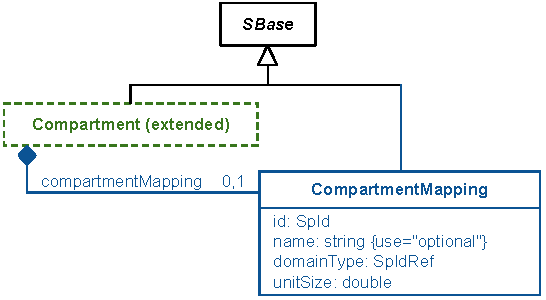
\includegraphics{figs/extended-compartment-uml}
  \caption{The definition of the extension to the \Compartment element, and the definition of the \CompartmentMapping class. The SBML core attributes of \Compartment are not displayed.}
  \label{compartment-uml}
  \label{CompartmentMapping-uml}
\end{figure}



The \Compartment element has an optional \CompartmentMapping child which indicates the \DomainType to which the \Compartment is mapped.  If there is no \CompartmentMapping for a \Compartment in a spatial model, then that \Compartment is excluded from the spatial version of the model.  In the same way, if a \DomainType is not mapped to one or more \Compartments, then the corresponding \Domains in the geometry have no assigned function.


\subsection{The \class{CompartmentMapping} class}
\label{CompartmentMapping-class}
Each \Compartment in a model that defines a spatial geometry may contain an optional \CompartmentMapping. A \CompartmentMapping is defined as part of the model rather than part of the geometry so that the geometry is modular and may be readily shared between models and reused.  A \CompartmentMapping maps a \Compartment defined in the model to a \DomainType defined in the geometry such that each corresponding \DomainType is assigned the same biological and mathematical function described by the set of \Compartments that are mapped to that \DomainType. 

This mapping need not be one-to-one.  In fact, it is common to map er-lumen, er-membrane, and cytosol to the same cell interior volume or 3D \DomainType.  The \token{unitSize} attribute specifies the relative quantity of each \Compartment that is mapped to the \DomainType.

\subsubsection{The \token{\changed{id}} attribute}
The \token{\changed{id}} attribute is a mandatory attribute of type \primtype{SpId} that is used to uniquely identify a \CompartmentMapping in the model.  All identifiers of type \primtype{SpId} must be unique within the \Geometry.  The mathematical value of a \CompartmentMapping is its \token{unitSize} attribute, and can be bound to a \Parameter by using a \SpatialSymbolReference.

\subsubsection{The \token{domainType} attribute}
The mandatory \token{domainType} attribute is of type \primtype{SpIdRef} that indicates a \DomainType defined in the \Geometry element.

\subsubsection{The \token{unitSize} attribute}
The \token{unitSize} attribute is of type \primtype{double} and represents the relative size of the \Compartment with respect to the size of the \Domains to which they are mapped.  Thus for any infinitesimal subset of the \Domain with size S, there exists an amount of Compartment$_{\text{i}}$ of size (S*unitSize$_{\text{i}}$) for i=1..N compartments mapped to that \DomainType.  For example, a 3D \Compartment (and \DomainType) which is mapped to a 3D \DomainType has a \token{unitSize} which is a volume fraction of dimensionless unit.  The total set of all such volume fractions mapped to a particular \DomainType will typically sum to one. 

If the \token{spatialDimensions} attribute of the parent \Compartment is different than the \token{spatialDimension} attribute of referenced \DomainType, the \token{unitSize} attribute is a conversion factor between the two.  The most common example of this would be a 2D \Compartment being mapped to a 3D \DomainType, such as an ER-membrane being mapped to a volumetric cell interior.  In this case, the \token{unitSize} is a surface-to-volume ratio.

If connected to a \Parameter via a \SpatialSymbolReference, an \InitialAssignment may override the value of the \token{unitSize} attribute.  It is theoretically possible to have this value change in time through the use of a \Rule or \Event, but some (if not all) software tools may not support this setup.  If the value is set to change, and the dimensionality of the parent \Compartment and referenced \DomainType is the same, the other \CompartmentMapping elements for the same \DomainType will typically change in concert, so that they continue to sum to one.

Any bound \Parameter's units should be equivalent to the units of the parent \Compartment divided by the units of the referenced \DomainType. 



\subsection{The extended \Species object}
\label{extended-species-class}
The SBML core \Species is extended when a spatial geometry is defined in the model with the addition of a single new required boolean \val{isSpatial} attribute.  The extension to the \Species element is shown in \fig{species-uml}.
 
\begin{figure}[ht]
  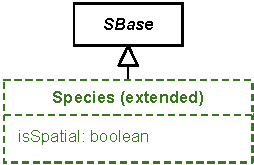
\includegraphics{figs/extended-species-uml}
  \caption{The extension to the \Species element. The attributes of \Species from \sbmlthreecore are not displayed.}
  \label{species-uml}
\end{figure}



\subsubsection{The \token{isSpatial} attribute}
The \token{isSpatial} attribute is of data type boolean. If it is set to true, the \Species is spatially distributed in a possibly nonhomogeneous manner within the \Domains of the same type as the mapped \DomainType. 

For continuous deterministic models (described by partial differential equations), a spatial \Species will result in a concentration field described by a partial differential equation which incorporates contributions from \Reactions, diffusion (\DiffusionCoefficient) and advection (\AdvectionCoefficient) and are subject to boundary conditions (\BoundaryCondition) and initial conditions (\InitialAssignment and \Rule).  All of these quantities can be explicit functions of the spatial coordinates as well as spatial and nonspatial \Parameters and \Species.  

For stochastic models, the \Species is represented as a collection of particles that are distributed throughout the \Domains and are subject to reactions, diffusion and advection.  Simulation algorithms either track individual particles (e.g. Particle-based methods) or use spatial discretization to track a large number of well stirred pools (e.g. Next-Subvolume Method).

The \token{compartment} of any \Species set \token{isSpatial} = \val{true} must have a child \CompartmentMapping: if it did not, its compartment would not actually be a part of the spatial model.


\subsection{The extended \Parameter object}
\label{extended-parameter-class}
When an SBML model defines a spatial geometry, the SBML core \Parameter is used to define the diffusion coefficient, transport velocity (advection) and boundary conditions for species and the coordinate components defined in the \Geometry. One \Parameter is created for each quantity, by adding a child \DiffusionCoefficient, \AdvectionCoefficient, or \BoundaryCondition.  Conversely, some elements defined in the spatial package may need to be referenced by mathematics in core constructs, or even have their value set by core constructs such as \InitialAssignment or \Rule.  These spatial elements can be semantically linked to a \Parameter by giving it a child \SpatialSymbolReference pointing to that element.

A \Parameter that has been extended for the Spatial package can have only one of the above listed objects.  For example, if a \Parameter is extended to represent the diffusion coefficient of a species, the existing attributes of the \Parameter (id, name, value, units, constant) are defined according to SBML core specifications, along with a \DiffusionCoefficient child that contains the information about the species it represents. \fig{parameter-uml} represents the extension to the \Parameter element.

\begin{figure}[ht]
  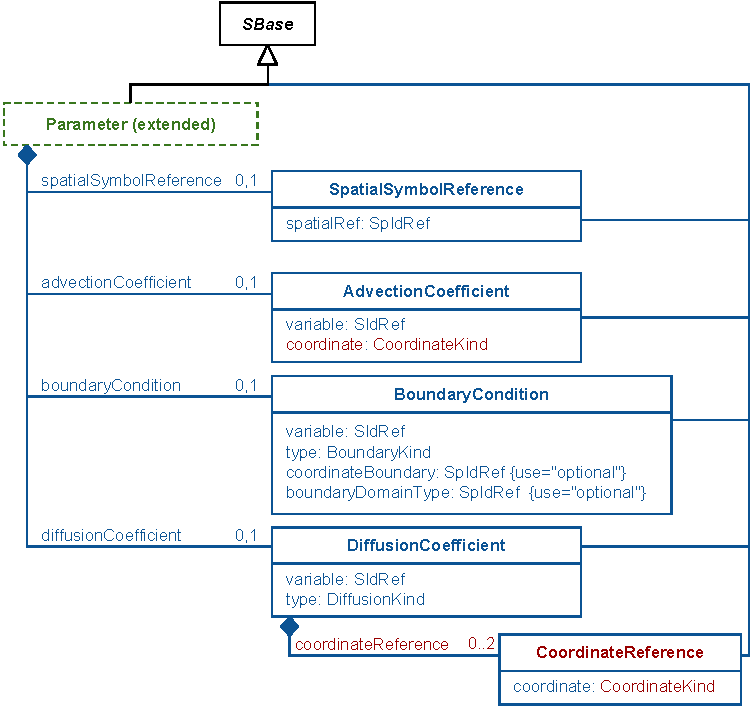
\includegraphics{figs/extended-parameter-uml}
  \caption{The \Parameter element extension for spatial package. The \sbmlthreecore attributes for \Parameter are not displayed in this figure.}
  \label{parameter-uml}
\end{figure}



\subsection{The \class{SpatialSymbolReference} class}
\label{SpatialSymbolReference-class}
A \Parameter is extended with a \SpatialSymbolReference element, when a symbol from the defined spatial geometry (\token{\changed{id}} of any element contained in \Geometry) is required to be used in the SBML core model. Typically, the \SpatialSymbolReference is used to represent the coordinate components defined in the \Geometry's listOfCoordinateComponents.  For example, if the \Geometry is defined in a 2-dimensional Cartesian coordinate system with X and Y defined as coordinate components, two \Parameters (one each for \CoordinateComponents X and Y) are created in the model. The value of the parameter is not required to be set. For each of these parameters, a \SpatialSymbolReference object is created.

\subsubsection{The \token{spatialRef} attribute}
The \token{spatialRef} attribute of \SpatialSymbolReference, is of type \primtype{SpIdRef} and refers to the \changed{\primtype{SpId}} of any element defined in the \Geometry of the model.

\subsection{The \class{DiffusionCoefficient} class}
\label{DiffusionCoefficient-class}
When a species in a spatial model has a diffusion rate constant, a \Parameter for this diffusion constant is created in the SBML model with a \DiffusionCoefficient child, which is used to identify the \Species whose diffusion rate the \Parameter represents. The diffusion coefficient can then be set like any other variable:  its initial value can be set using the \Parameter's \token{value} attribute or through an \InitialAssignment, and if the diffusion coefficient changes in time, this can be defined with a \Rule or \Event. If set, the units of this \Parameter should be length$^2$/time.  If left unset, the \DiffusionCoefficient will inherit the model units of length$^2$/time (typically cm$^2$s$^{-1}$ or um$^2$s$^{-1}$).


It is possible to define both diffusion and advection for the same \Species.

\subsubsection{The \token{variable} attribute}
The required \token{variable} attribute of \DiffusionCoefficient is of type \primtype{SIdRef} and is the \primtype{SId} of the \Species or \Parameter in the model whose diffusion coefficient is being set.

\subsubsection{The \token{type} attribute}
The required \token{type} attribute of \DiffusionCoefficient is of type \primtype{DiffusionKind} and indicates whether the diffusion coefficient is \val{isotropic} (i.e. applies equally in all dimensions/directions) \val{tensor} (i.e. applies only for a particular pair of coordinates), \changed{or \val{anisotropic} (i.e. applies only for a single coordinate)}.  Coefficients of type \val{isotropic} may not have any child \changed{\CoordinateReference} children; coefficients of type \val{tensor} must have exactly two; \changed{and coefficients of type \val{anisotropic} must have exactly one}.


\subsubsection{The \class{\changed{CoordinateReference}} class}
\label{CoordinateReference-class}
The optional \changed{\CoordinateReference} children of the \DiffusionCoefficient object contain \changed{(in their own \token{coordinate} attribute)} the \changed{type} attributes of the \CoordinateComponent (e.g. \changed{\val{cartesianX}, \val{cartesianY}, or \val{cartesianZ}}), for specifying axis or axes it applies to.

\begin{blockChanged}
If the \DiffusionCoefficient has two \CoordinateReference children, the diffusion coefficient is defined for flux in the plane defined by the two \changed{\CoordinateReference} axes.  The diffusion is defined in relation to the direction due to a gradient in the diagonal term of the diffusion tensor for the two coordinates.

If the \DiffusionCoefficient has exactly one \CoordinateReference child, the diffusion is considered to be anisotropic. To be complete, one \DiffusionCoefficient will need to be defined per axis.

If the \DiffusionCoefficient has no \CoordinateReference children, the diffusion is considered to be Isotropic.
\end{blockChanged}

{\color{red} Lucian: \notice Updated again, but still potentially in flux.  We probably need more text here in general to describe the situation.}

\subsubsection{\DiffusionCoefficient uniqueness}
Only one \DiffusionCoefficient may be defined per \Species per pair of valid axes in the \Compartment in which it resides.  Since isotropic diffusion is defined for all axes at once, this means that if an isotropic \DiffusionCoefficient is defined for a \Species, it may have no other diffusuion coefficients.


\subsection{The \class{AdvectionCoefficient} class}
\label{AdvectionCoefficient-class}
The \AdvectionCoefficient is the extension to \Parameter in SBML core that is used to represent transport velocity of a species, if it exists. The transport velocity for the species is defined in a manner similar to the diffusion constant with a unit of length/time (regardless of the units of the corresponding \Species' \val{compartment} attribute).  A \Parameter is created in SBML code for the velocity with an \AdvectionCoefficient child to identify the \Species whose velocity is represented by the \Parameter; its initial value is set either through the \token{value} attribute or an \InitialAssignment.    If the advection coefficient changes in time or space, this can be modeled with a \Rule or \Event.

If defined, the units of the parent \Parameter should be in length/time; if not defined, it inherits from the model-wide units of length divided by the model-wide units of time.

It is possible to define both diffusion and advection for the same \Species.

\subsubsection{The \token{variable} attribute}
The \token{variable} attribute of \AdvectionCoefficient is of type \primtype{SIdRef} and is the SId of the \Species or \Parameter in the model whose advection coefficient (transport velocity) is being set.

\subsubsection{The \token{\changed{coordinate}} attribute}
The \token{\changed{coordinate}} is of type \changed{\primtype{CoordinateKind}} and represents the coordinate component of the velocity. For example, if the \Geometry is defined in the Cartesian coordinate system and is 2-dimensional, the species can have velocity terms for both X and Y. If the \Parameter represents the transport velocity of the species in the X-coordinate, the \token{\changed{coordinate}} attribute will take a value of \changed{\val{cartesianX}}, and if it represents the velocity in the Y-coordinate, the attribute will take a value of \changed{\val{cartesianY}}.  Only one \AdvectionCoefficient may be defined per \Species per valid \token{\changed{coordinate}}.

{\color{red} Lucian: \notice Changed to CoordinateKind.}


\subsection{The \class{BoundaryCondition} class}
\label{BoundaryCondition-class}
A \Species in a spatial model that has a diffusion rate or an advection velocity needs to have specified boundary conditions. A boundary condition is either the concentration of the species or the flux density of the species at a boundary.  The boundary refers to either an internal membrane boundary or a face of the box defined by the minimum and maximum coordinates of the geometry (the geometries bounding box).  

When creating a spatial SBML model, species boundary conditions are created as parameters, one for each boundary condition, by adding a child \BoundaryCondition that points to the corresponding \Species and boundary, depending on the coordinate system.


For Cartesian Geometries, there are two boundaries for every axis being modeled.  For example, in a 2D cartesian geometry for the external boundaries, there could be up to four parameters or parameter sets created for each spatial \Species whose \Compartments abut the minimum and maximums of the X and Y axes).

%For polar and cylendrical Geometries, there is one boundary for the maximum of the radius, and another boundary for the minimum of the radius if that minimum is not \val{0}.  For the azimuth, there are either two boundaries corresponding to the minimum and maximum azimuth, or no boundaries, if the minimum is 0$^\circ$, and the maximum is 360$^\circ$.  In cylendrical geometry, there will be two boundaries for the minumum and maximum height.

%For spherical Geometries, there will again be one boundary for the maximum of the radius, and another boundary for the minumum of the radius if that minimum is not \val{0}.  For the spherical azimuth and elevation, there will be either two boundaries each corresponding to the minimum and maximum values, or no boundaries, for each minimum 0$^\circ$ and maximum 360$^\circ$ pair.

The \Parameter's value is set either through the \token{value} attribute or an \InitialAssignment.  If the boundary condition changes in time, it can be set with a \Rule or \Event.  If set, the \Parameter unit must be equal to the appropriate unit for its \token{type} (see below).  Only one \BoundaryCondition may be defined per \Species per boundary (regardless of type).


\subsubsection{The \token{variable} attribute}
The \token{variable} attribute of \BoundaryCondition is of type \primtype{SIdRef} and is the SId of the \Species or \Parameter in the model whose boundary condition is being set.

\subsubsection{The \token{type} attribute}
The \token{type} attribute is of type \primtype{BoundaryConditionKind} and indicates the type of boundary condition. The boundary condition types come in three groups: for Neumann boundaries, \changed{\val{Neumann} (the inward normal flux)} is used.  For Dirichlet boundaries, \changed{\val{Dirichlet} (the value)} is used.  For Robin boundaries, three different Parameters must be defined, with \BoundaryCondition elements of type \val{Robin\_valueCoefficient}, \val{Robin\_inwardNormalGradientCoefficient}, and \val{Robin\_sum}.

The unit of the boundary condition is determined by the type, and the unit for density and velocity.  For \val{\changed{Dirichlet}}, the unit would be the unit of concentration.  For \val{\changed{Neumann}}, the unit would be concentration*length/time.  For Robin boundaries, for a variable \val{u} with an inward pointing normal vector \val{n}, Robin value coefficient \val{a}, Robin inward normal gradient coefficient \val{b}, and Robin sum \val{g}, the condition is defined by the equation \val{a*u + b*inner\_product(grad(u),n) = g}, with appropriate units.

{\color{red} Lucian: \notice Does this explanation work?}

\subsubsection{The \token{coordinateBoundary} attribute}
The \token{coordinateBoundary} attribute is of type \primtype{SpIdRef} and refers to the \changed{\primtype{SpId}} of either the \token{boundaryMin} or \token{boundaryMax} object of the \CoordinateComponent defined in \Geometry. This \changed{\primtype{SpId}} indicates the boundary condition (minimum or maximum) in the \CoordinateComponent. A \Parameter that is extended with a \BoundaryCondition object can only define the \token{coordinateBoundary} attribute or the \token{boundaryDomainType} attribute, but not both.

\subsubsection{The \token{boundaryDomainType} attribute}
The \token{boundaryDomainType} attribute is of type \primtype{SpIdRef} and refers to the \changed{\primtype{SpId}} of the \DomainType of the location of the species whose boundary condition is being defined. A \Parameter that is extended with a \BoundaryCondition object can only define the \token{coordinateBoundary} attribute or the \token{boundaryDomainType} attribute, but not both. 


\subsection{The extended \Reaction object}
\label{extended-reaction-class}
The SBML core \Reaction is extended when a spatial geometry is defined in the model with the addition of a single new required boolean \token{isLocal} attribute. \fig{reaction-uml} displays the definition of the extension of the \Reaction element.
 
\begin{figure}[ht]
  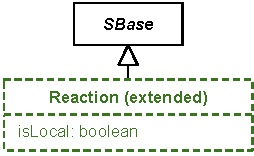
\includegraphics{figs/extended-reaction-uml}
  \caption{The extension to the \Reaction element. The \sbmlthreecore atrributes and children for \Reaction are not displayed in the figure.}
  \label{reaction-uml}
\end{figure}

\subsubsection{The \token{isLocal} attribute}
The \token{isLocal} attribute for a \Reaction is of type \primtype{Boolean}. The attribute is set to true if the reaction is to be considered a local description of the reaction in terms of concentration/time defined at each point in space rather than substance/time over an entire \Compartment or "pool".  Note that this means that the units of the \KineticLaw are different depending on whether the \Reaction is local or not.


\subsection{The \class{Geometry} class}
\label{Geometry-class}
\label{ListOfCoordinateComponents-class}
\label{ListOfDomainTypes-class}
\label{ListOfDomains-class}
\label{ListOfAdjacentDomains-class}
\label{ListOfGeometryDefinitions-class}

A single geometry must be defined within the model if the spatial extension is to be used. \fig{Geometry-uml} shows the definition of the \Geometry element.
 
\begin{figure}[ht]
  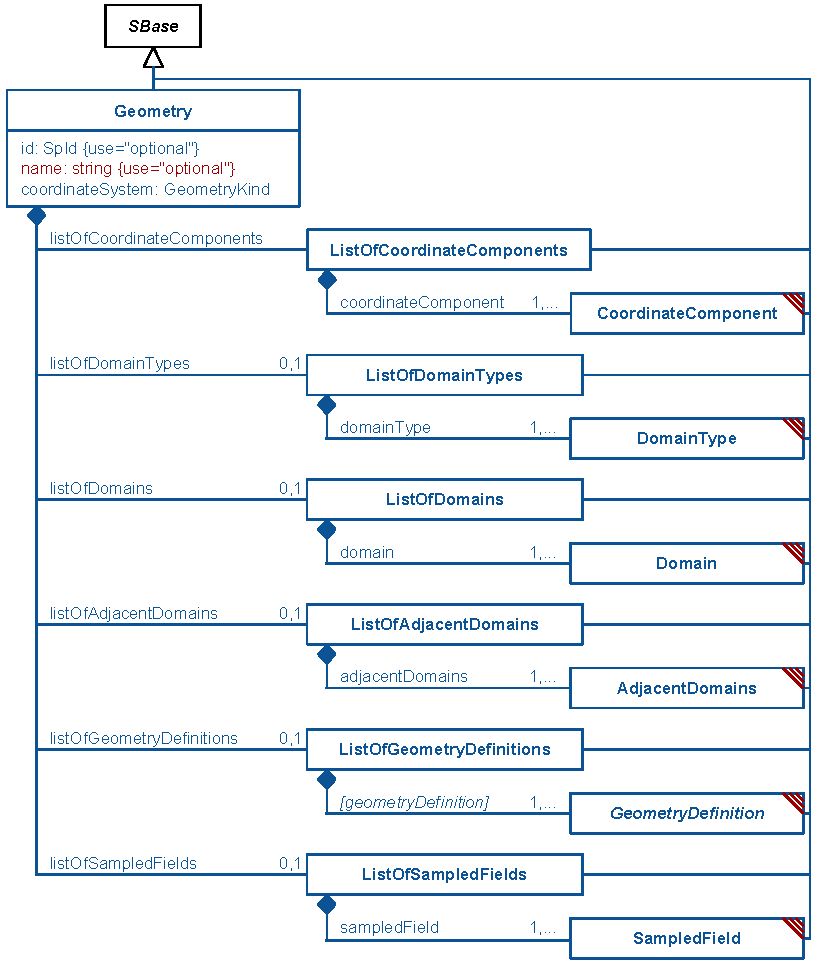
\includegraphics{figs/Geometry-uml}
  \caption{The definition of the \Geometry, \ListOfCoordinateComponents, \ListOfDomainTypes, \ListOfDomains, \ListOfAdjacentDomains, and \ListOfGeometryDefinitions classes from the Spatial package.  The various children of the ListOf- classes are defined in their own sections.}
  \label{Geometry-uml}
  \label{ListOfCoordinateComponents-uml}
  \label{ListOfDomainTypes-uml}
  \label{ListOfDomains-uml}
  \label{ListOfAdjacentDomains-uml}
  \label{ListOfGeometryDefinitions-uml}
\end{figure}

\subsubsection{The \token{\changed{id}} attribute}
The \token{\changed{id}} attribute is of type \primtype{SpId}, uniquely identifies the \Geometry element, and is optional.  It has no mathematical meaning.

\subsubsection{The \token{coordinateSystem} attribute}
The \token{coordinateSystem} attribute is a required attribute and is of type \primtype{GeometryKind}. It represents the coordinate system used by the \Geometry.  A value of  \val{cartesian} indicates that the geometry is a cartesian coordinate system, with the coordinate components corresponding to the x, y, and z components of that system (which could be 1-, 2-, or 3-dimensional).  This is the only coordinate system defined in this version of the specification--in the future, if necessary, \val{cylendrical}, \val{spherical}, and \val{polar} may be added as possibilities, along with n-dimensional cartesian modeling, should there be interest in the modeling community to exchange these types of models.

%A value of \val{cylindrical} indicates that the geometry is a three-dimensional cylendrical coordinate system, with coordinate components corresponding to radial distance, azimuth angle, and axial position.  A value of \val{spherical} indicates that the geometry is a three-dimensional spherical coordinate system, with coordinate components corresponding to radial distance, polar angle, and azimuth angle.  A value of \val{polar} indicates that the geometry is a two-dimensional polar coordinate system, with coordinate components corresponding to radial distance and angle (the two-dimensional equivalent of the cylendrical coordinate system).

\subsubsection{The listOf container classes}
The \Geometry has listOfCoordinateComponents, listOfDomainTypes, listOfDomains, and listOfAdjacentDomains, and listOfGeometryDefinitions that help define the geometry.  The \ListOfCoordinateComponents is a list of \CoordinateComponent objects, the \ListOfDomainTypes is a list of \DomainType objects, the \ListOfDomains is a list of \Domain objects, \ListOfAdjacentDomains is a list of \AdjacentDomains objects, and the \ListOfGeometryDefinitions is a list of alternative \GeometryDefinitions (\ParametricGeometry,\CSGeometry, \SampledFieldGeometry, \AnalyticGeometry).  None of these lists are technically required, but, if present, none of them may be empty.

Note that the children of the \ListOfGeometryDefinitions object are not called \token{geometryDefinition} but rather take the name of the derived class, decapitalized.  Thus, they may be called \token{parametricGeometry}, \token{sampledFieldGeometry}, \token{csGeometry}, or \token{analyticGeometry}.


\subsection{The \class{CoordinateComponent} class}
\label{CoordinateComponent-class}
A \CoordinateComponent object explicitly defines a coordinate component of the coordinate axes and gives them names, units, and formally associates them with a coordinate system. The \CoordinateComponent also defines the minimum and maximum values of the coordinate axis it represents. The definition of \CoordinateComponent is shown in \fig{CoordinateComponent-uml}.
 
\begin{figure}[ht]
  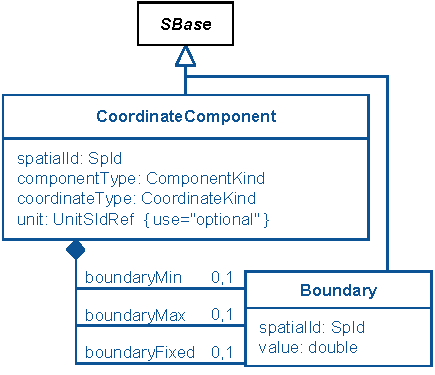
\includegraphics{figs/CoordinateComponent-uml}
  \caption{The \CoordinateComponent object definition. One or more instances of \CoordinateComponent objects in a \ListOfCoordinateComponents can be present in \Geometry.}
  \label{CoordinateComponent-uml}
\end{figure}


\subsubsection{The \token{\changed{id}} attribute}
A \CoordinateComponent is identified with the \token{\changed{id}} attribute which is of type \primtype{SpId}.  When referenced (for example, via a \SpatialSymbolReference extension of the SBML core \Parameter object) and used within a mathematical expression, it represents the coordinate value for this \CoordinateComponent.
 
Because a \CoordinateComponent represents an entire axis, it is not appropriate, should it be connected to a \Parameter via a \SpatialSymbolReference, for that \Parameter to be set via an \InitialAssignment or \Rule.  Rather, it is treated like the SBML core \token{csymbol} \val{time}, and can be used as an independent variable in other calculations.

\subsubsection{The \token{\changed{type}} attribute}
The \token{\changed{type}} attibute of type \primtype{\changed{CoordinateKind}} represents the type of the coordinate component, and may take one of a subset of all possible \primtype{\changed{CoordinateKind}} values depending on its parent \Geometry, as defined in \tab{CoordinateComponent-Geometry-relation}.
%For all \primtype{GeometryKind} values except \val{cartesian}, exactly one \CoordinateComponent must exist with each of the allowed \primtype{\changed{CoordinateKind}} values:  in other words, a \val{cylendrical} \Geometry must have exactly three \CoordinateComponent children, each one having a different allowed value for its \token{\changed{type}} attribute.
For Cartesian geometries, one-dimensional geometries may be defined by having a single \val{cartesianX} \CoordinateComponent; two-dimensional geometries may be defined by having two \CoordinateComponent children with \token{\changed{type}} values of \val{cartesianX} and \val{cartesianY}, and three-dimensional geometries may be defined by having three \CoordinateComponent children with \token{\changed{type}} values of \val{cartesianX}, \val{cartesianY}, and \val{cartesianZ}.

\begin{table}[thb]
  \begin{edtable}{tabular}{>{\centering\arraybackslash}m{0.9in} >{\centering\arraybackslash}m{0.7in} >{\raggedright\arraybackslash}m{4.4in}}
  %\begin{edtable}{tabular}{p{0.9in}p{0.7in}p{4.4in}}
    \toprule
    \textbf{GeometryKind} & \textbf{Dimensions} & \textbf{\changed{CoordinateKind}s} \\
    \midrule
    \token{cartesian}   & 1 & \val{cartesianX} (\token{coord1})\\
    \token{cartesian}   & 2 & \val{cartesianX} (\token{coord1}) and \val{cartesianY} (\token{coord2})\\
    \token{cartesian}   & 3 & \val{cartesianX} (\token{coord1}), \val{cartesianY} (\token{coord2}), and \val{cartesianZ} (\token{coord3})\\
 %   \token{cylendrical} & 3 & \val{cylindricalRadius} (\token{coord1}), \val{cylindricalAzimuth} (\token{coord2}), and \val{cylindricalHeight} (\token{coord3})\\
 %   \token{polar}       & 2 & \val{polarRadius} (\token{coord1}) and \val{polarAzimuth} (\token{coord2})\\
 %   \token{spherical}   & 3 & \val{sphericalRadius} (\token{coord1}), \val{sphericalAzimuth} (\token{coord2}), and \val{sphericalElevation} (\token{coord3})\\
    \bottomrule
  \end{edtable}
  \caption{Correspondance between the \token{type} of a \Geometry and the possible \token{\changed{type}}s of its child \CoordinateComponent elements.  Also noted is the corresponding attribute (\token{coord1}, \token{coord2}, or \token{coord3}) corresponding to each axis when defining \InteriorPoint elements (see \sec{InteriorPoint-class}).} 
  \label{CoordinateComponent-Geometry-relation}
\end{table}



%\subsubsection{The \token{coordinateType} attribute}
%The \token{coordinateType} attribute, of type \primtype{CoordinateKind}, represents whether the axis being defined is normal (\val{normal}), or whether it represents a dimension that does not need to be modeled explicitly in any performed calculations, whether due to symmery, where the modeled element exists in the given dimension, but is assumed to be the same for all values along that axis (\val{symmetrical}), or due to being constrained to a single value along that axis (\val{fixed}).

%\CoordinateComponent elements of coordinateType \val{normal} must have a \token{boundaryMin} and \token{boundaryMax} child.  \CoordinateComponent elements of coordinateType \val{symmetrical} may have a \token{boundaryMin} and \token{boundaryMax} children for visualization purposes, but they are optional.  \CoordinateComponent elements of coordinateType \val{fixed} must have a single \token{boundaryFixed} child.

{\color{red} Lucian: \notice coordinateType attribute removed.}


\subsubsection{The \token{unit} attribute}
The unit of a \CoordinateComponent is represented by the \token{unit} attribute, of type \primtype{UnitSIdRef}.  If not specified, the unit of a \CoordinateComponent inherits from the \token{lengthUnits} attribute of the \Model object, and if that in turn is not specified, the \CoordinateComponent units cannot be determined.
%Many coordinates may have different units from the \token{lengthUnits} of the \Model, since this is a distance metric and not always the same as the unit of each individual coordinate.  For example, in Polar coordinates, the coordinate component 'theta' may be described in radians while component 'rho' may be in microns.  


\subsection{The \class{Boundary} class}
\label{Boundary-class}
The minimum and the maximum for a \CoordinateComponent represent the bounds in each coordinate.  For example, for three dimensional Cartesian coordinate system with x, y, and z coordinates, the minimum and maximum limits for each coordinates define planes orthogonal to each coordinate axis and passing through the minimum or maximum.  If max-min is the same for each x,y,z then the bounds on the geometry is a cube.  The \Boundary class interacts with the \BoundaryCondition class, allowing modelers to define how model elements behave at the boundary of the model.  For species defined within volumes adjacent to these surfaces, \BoundaryCondition elements must be introduced.

{\color{red} Lucian: \notice Just a note to coordinate the text here to sync with the text in the \BoundaryCondition class, if that changes.  }

The minimum limit of a \CoordinateComponent is represented by the \token{boundaryMin} object and the maximum limit is represented by the \token{boundaryMax} object, and apply to \CoordinateComponent elements.
%of coordinateType \val{normal} and \val{symmetrical} (and are optional in the latter case only).
Both are \Boundary objects, and have the following attributes:

%For \CoordinateComponent elements of coordinateType \val{fixed}, a single \token{boundaryFixed} object defines the value at which the coordinate component is fixed.  

\subsubsection{The \token{\changed{id}} attribute}
The \token{\changed{id}} attribute of the \Boundary object identifies the object. The attribute is required and is of type \primtype{SpId}. This attribute is used when specifying the \BoundaryCondition for a species as an extension of an SBML core \Parameter.   When referenced (for example, via a \SpatialSymbolReference extension of the SBML core \Parameter object) and used within a mathematical expression, it represents the value of the \Boundary.  The units are the same as its parent \CoordinateComponent, and are not set separately.

\subsubsection{The \token{value} attribute}
The \token{value} attribute is of type \primtype{double}. In a \token{boundaryMin} object, it represents the minimum limit of the \CoordinateComponent.  In a \token{boundaryMax} object, it represents the maximum limit of the \CoordinateComponent.

%In a \token{boundaryFixed} object, it represents the fixed level of the \CoordinateComponent.

If connected to a \Parameter via a \SpatialSymbolReference, this \token{value} may be overridden by an \InitialAssignment.  It is theoretically possible to have this value change in time through the use of a \Rule or \Event, but some (if not all) software tools may not support this setup. 


\subsection{The \class{DomainType} class}
\label{DomainType-class}
A \DomainType is a class of domains that are identified as being anatomically and physiologically similar.  For example, a \DomainType "cytosol" may be defined in a \Geometry as identifying the structure and function of the cell interior.  If there is one cell, then there is one domain, if there are multiple cells, then there are multiple disjoint domains ("cytosol1","cytosol2", etc.) identified with the \DomainType "cytosol".  \CompartmentMappings, defined as an extension to an SBML core \Compartment, map compartments to domain types such that each corresponding domain is assigned the same biological and mathematical function. \fig{DomainType-uml} shows the \DomainType object.

Each SBML \Compartment maps to a single \DomainType, meaning that the initial condition of each \Species in each \Compartment will be the same across all \Domains that map to a given \DomainType.  If those \Species are spatially distributed, they will subsequently evolve independently from each other.  However, if modeling two \Domains that are similar but whose \Species have different initial conditions, those \Domains should be modeled as separate \DomainTypes.

\begin{figure}[ht]
  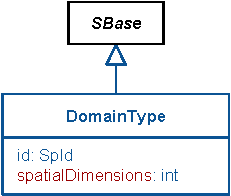
\includegraphics{figs/DomainType-uml}
  \caption{The \DomainType object. One or more instances of \DomainType in a \ListOfDomainTypes instance can be present in a \Geometry object.}
  \label{DomainType-uml}
\end{figure}

\subsubsection{The \token{\changed{id}} attribute}
Each \DomainType is identified with a \token{\changed{id}} of type \primtype{SpId}.  When referenced and used within a mathematical expression, it represents the sum of the sizes of all domains associated with this \DomainType.

As a derived quantity, if connected to a \Parameter via a \SpatialSymbolReference, this value may \emph{not} be overridden by an \InitialAssignment, nor by the use of a \Rule or \Event.  Its value is always connected to the size of its component \Domains instead.  The units of a \DomainType are the units of the corresponding base units of the SBML \Model for length (for one-dimensional domains), area (for two-dimensional domains), or volume (for three-dimensional domains).  It is required to define the corresponding base units for every \DomainType in the \Model.

\subsubsection{The \token{spatialDimension} attribute}
The \token{spatialDimension} attribute of the \DomainType is of type \primtype{int} and can take on a value of 0, 1, 2, or 3. The spatial dimension is specified for a \DomainType, rather than being repeated for each \Domain that is represented by the \DomainType.

{\color{red} Lucian: \notice The equivalent attribute of a \Compartment is \token{spatialDimensions}, i.e. it has an 's' on the end.  Can we change this to match?}


\subsection{The \class{Domain} class}
\label{Domain-class}
\label{ListOfInteriorPoints-class}
\Domains represent contiguous regions identified by the same \DomainType.  One, two and three dimensional domains are contiguous linear regions, surface regions, and volume regions (respectively), bounded by the limits of the coordinate system (e.g. min/max of x,y,z) and adjacent domains corresponding to different domain types.  \Domain is shown in \fig{Domain-uml}.
 
\begin{figure}[ht]
  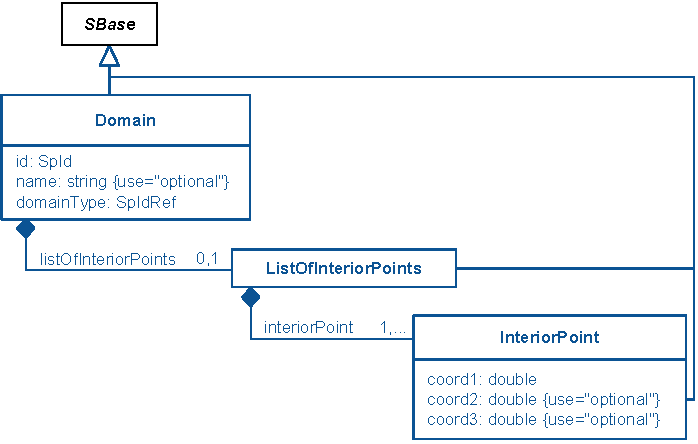
\includegraphics{figs/Domain-uml}
  \caption{The definition of the \Domain, \ListOfInteriorPoints, and \InteriorPoint classes.  A \ListOfDomains instance in \Geometry can contain one or more \Domain object instances.}
  \label{Domain-uml}
  \label{InteriorPoint-uml}
  \label{ListOfInteriorPoints-uml}
\end{figure}

\subsubsection{The \token{\changed{id}} attribute}
A \Domain is identified with an \changed{\token{id}} attribute of type \primtype{SpId}.  This \token{\changed{id}} may be used within a \SpatialSymbolReference object that is extended from an SBML core \Parameter and can be used in an expression.  When referenced, the domain evaluates to the absolute size of that domain as used by the simulator (the meshed size).

As a derived quantity, if connected to a \Parameter via a \SpatialSymbolReference, this value may \emph{not} be overridden by an \InitialAssignment, nor by the use of a \Rule or \Event.  Its value is always connected to the size of the corresponding \Geometry instead.  The units of the \Domain are the same as the units of the corresponding \DomainType.

\subsubsection{The \token{domainType} attribute}
The \token{domainTpe} attribute refers to the \changed{\primtype{SpId}} of the \DomainType that describes the anatomy and physiology of this domain. The attribute is of type \primtype{SpIdRef}. It is through this association that compartments, and hence the whole SBML model, gets mapped to the individual domains. 


\subsection{The \class{InteriorPoint} class}
\label{InteriorPoint-class}
Each \Domain can contain a \ListOfInteriorPoints. The list of spatial points for a domain is interior to that domain.  This list is optional for a \Domain if it is the only \Domain defined for its \DomainType, but is required otherwise.

For those geometric descriptions that can describe multiple disjoint domains belonging to the same \token{domainType}, these interior points allow unambiguous identification of each domain.  Formally, a single point would suffice, but in practice some tools (e.g. Smoldyn) require multiple points to handle non-convex volumes bounded by explicit surfaces.  For discontinuous surfaces with the same \token{domainType}, the interior point identifies which domain is associated with which surface patch defined in the geometry definition.

Each \InteriorPoint has three attributes: \token{coord1}, \token{coord2}, and \token{coord3}. 

\subsubsection{The \token{coord1}, \token{coord2}, and \token{coord3} attributes}
An InteriorPoint element represents a single point within the defined coordinate system and should be in the interior of the domain that contains it. It has three attributes, \token{coord1}, \token{coord2}, and \token{coord3}, of type \primtype{double}, representing the position along each of the up to three coordinate axes defined by the \CoordinateComponents \changed{(with \token{type} \val{cartesianX}, \val{cartesianY}, and \val{cartesianZ}, respectively, for each \token{coord\_} attribute}; see \tab{CoordinateComponent-Geometry-relation}).

Each \InteriorPoint must define the same number of attributes as there are dimensions of the corresponding \Geometry to which it belongs.

In the case of surfaces, interior points are sometimes required to make unambiguous identification of multiple surfaces (e.g multiple plasma membranes for multiple cells present in a geometry).  Due to roundoff error and finite word lengths, it is difficult to find a three dimensional point that lies on a surface.  In this case, the distance from the surface will be used to provide unambiguous identification.


\subsection{The \class{AdjacentDomains} class}
\label{AdjacentDomains-class}
\AdjacentDomains (or domain adjacencies) captures the topological relationships within the \Geometry.  Consider that the \Domains are nodes in a graph. The \AdjacentDomains objects are the edges that specify the spatial connectivity of these nodes.  Armed with the topology and the domain sizes, one can readily perform a compartmental approximation.  \fig{AdjacentDomains-uml} shows the definition of the \AdjacentDomains object.

\begin{figure}[ht]
  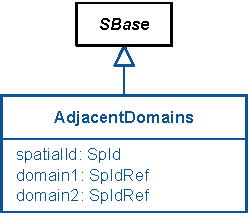
\includegraphics{figs/AdjacentDomains-uml}
  \caption{The definition of the \AdjacentDomains class. \Geometry can contain one instance of \ListOfAdjacentDomains that can have one or more instances of \AdjacentDomains objects.}
  \label{AdjacentDomains-uml}
\end{figure}

\subsubsection{The \token{\changed{id}} attribute}
This attribute identifies an \AdjacentDomains object. The attribute is of type \primtype{SpId}.  It has no mathematical meaning.

\subsubsection{The \token{domain1} and \token{domain2} attributes}
The \token{domain1} and \token{domain2} attributes, of type \primtype{SpIdRef}, are required attributes. They are the \changed{\primtype{SpId}}'s of two domains that touch each other (spatially adjacent).  These are typically surface-volume contacts.


\subsection{The \class{GeometryDefinition} class}
\label{GeometryDefinition-class}
A \Geometry can specify a list of \GeometryDefinitions. The \GeometryDefinition is an abstract class that is the general term for the container which defines the concrete geometric constructs represented by the \Geometry. Four types of \GeometryDefinitions have been identified - \AnalyticGeometry, \SampledFieldGeometry, \ParametricGeometry, \CSGeometry (Constructed Solid Geometry) - and are elaborated in the following sections. The definition of the \GeometryDefinition element is displayed in \fig{GeometryDefinition-uml}.  The spatial dimension of the \GeometryDefinition must match the \token{spatialDimension} of the \DomainType defined for the associated \Domain.

\begin{figure}[ht]
  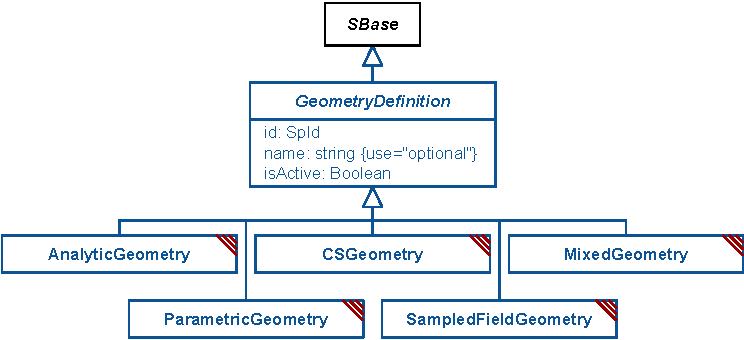
\includegraphics{figs/GeometryDefinition-uml}
  \caption{The \GeometryDefinition element. \Geometry contains one instance of listOfGeometryDefinitions that can contain one or more instances of \GeometryDefinition (one of \AnalyticGeometry, \SampledFieldGeometry, \CSGeometry, \ParametricGeometry, defined below).}
  \label{GeometryDefinition-uml}
\end{figure}

\subsubsection{The \token{\changed{id}} attribute}
The \token{\changed{id}} attribute that is common to all the \GeometryDefinition types is used to uniquely identify the \GeometryDefinition. The attribute is of type \primtype{SpId}.  A \GeometryDefinition has no mathematical meaning.


\subsection{The \class{AnalyticGeometry} class}
\label{AnalyticGeometry-class}
\label{ListOfAnalyticVolumes-class}
The \AnalyticGeometry is a class of \GeometryDefinition where the geometry of each domain is defined by an analytic expression. An \AnalyticGeometry is defined as a collection of \AnalyticVolumes, one \AnalyticVolume for each volumetric domain in the geometry. In this representation, the surfaces are treated as the boundaries between dissimilar \AnalyticVolumes. The \AnalyticGeometry object contains a \ListOfAnalyticVolumes. \fig{AnalyticGeometry-uml} shows the definition of the \AnalyticGeometry object.

\begin{figure}[ht]
  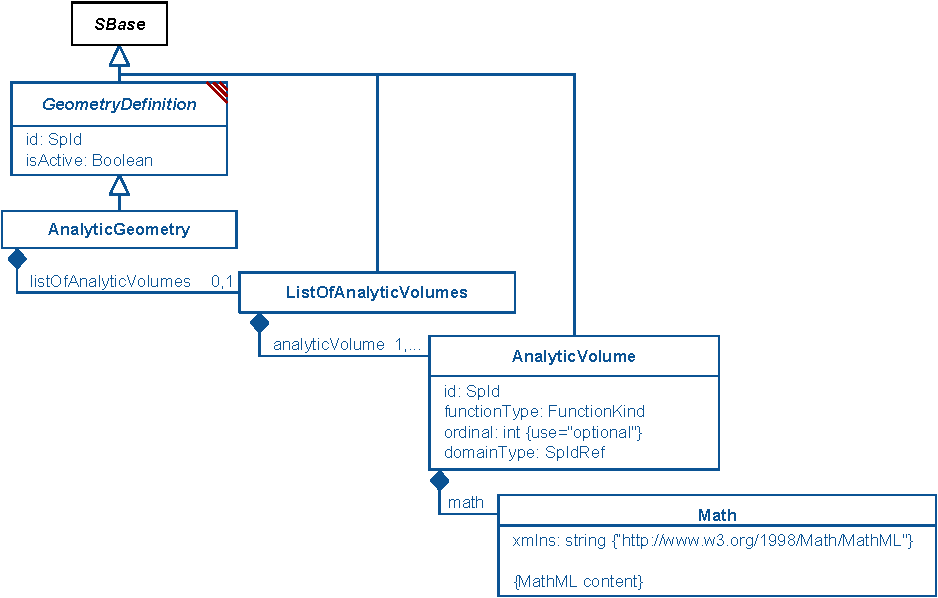
\includegraphics{figs/AnalyticGeometry-uml}
  \caption{The definition of the \AnalyticGeometry, \ListOfAnalyticVolumes, and \AnalyticVolume classes.}
  \label{AnalyticGeometry-uml}
  \label{ListOfAnalyticVolumes-uml}
  \label{AnalyticVolume-uml}
\end{figure}


\subsection{The \class{AnalyticVolume} class}
\label{AnalyticVolume-class}
The \AnalyticVolume is used to specify the analytic expression of a volumetric (3-dimensional) domain. The analytic expression for the \AnalyticVolume is defined in the Math element.

\subsubsection{The \token{\changed{id}} attribute}
The \token{\changed{id}} attribute uniquely identifies the \AnalyticVolume. The attribute is required and is of type \primtype{SpId}.  It has no mathematical meaning.

\subsubsection{The \token{functionType} attribute}
The \token{functionType} attribute is of type \primtype{FunctionKind} and is currently limited to just \val{layered} \changed{(a possibility for future versions of the specification is to allow the value \val{R-function})}.  A \val{layered} function type implies that the Math child element contains an inequality in the spatial dimensions (e.g. x,y,z) such that evaluation to \val{true} indicates that the point (x,y,z) is within that shape, and "false" indicates that it is not covered by that shape.
%The \val{R-function} \token{functionType} indicates that the shape is represented by a real-valued function whose sign indicates coverage by the shape.

{\color{red} Lucian: \notice If you want to rename 'layered', now is the time to do it ;-)}

\subsubsection{The \token{domainType} attribute}
The \token{domainType} attribute of type \primtype{SpIdRef} is a required attribute. It represents the \changed{\primtype{SpId}} of the \DomainType of the \Domain that is represented by this \AnalyticVolume. 

\subsubsection{The \token{ordinal} attribute}
The \token{ordinal} attribute of type \primtype{int} is an optional attribute. It is used to represent the order of the \AnalyticVolume. The \token{ordinal} is useful while reconstructing the geometry in the specific software tool - it represents the order in which the \AnalyticVolumes representing geometric domains have to be evaluated.

Rather than struggle with the task of preventing overlapping regions of space from different \AnalyticVolumes, the \AnalyticVolumes are to be considered to be evaluated in the reverse order of their ordinals.  In this way, any \AnalyticVolumes that have already been processed will cover those with a smaller ordinal, thus resolving any ambiguities and removing the constraint that all \AnalyticVolumes be disjoint and cover the entire geometric domain.  The \AnalyticVolume with \token{ordinal} 0 can be the "background" layer (typically the extracellular space).  

No two \AnalyticVolumes may have the same \token{ordinal} value, even if they should not overlap, because some tools may not calculate the geometries to the same level of precision as other tools, and may end up with overlap due to rounding errors, and will still need to resolve the ambiguity for their own purposes.  Any \AnalyticVolume without an \token{ordinal} value should also not overlap with any other \AnalyticVolume, but if it does, the software tool may resolve the situation however it sees fit.


\subsection{The \class{Math} class}
\label{Math-class}
The Math element is a required element for an \AnalyticVolume. The Math element contains a MathML expression that defines the analytic expression for the \AnalyticVolume referencing the coordinate components that are specified in the \ListOfCoordinateComponents in the \Geometry, according to the \token{functionType}. 


\subsection{The \class{SampledFieldGeometry} class}
\label{SampledFieldGeometry-class}
\label{ListOfSampledVolumes-class}
\SampledFieldGeometry is a type of \GeometryDefinition that defines a sampled image-based geometry or a geometry based on samples from a level set. \SampledFieldGeometry is defined using a \SampledField that specifies the sampled image and a list of \SampledVolumes that represent the volumetric domains as sampled image regions. \fig{SampledFieldGeometry-uml} shows the definition of the \SampledFieldGeometry object.  It may be used for geometries of any dimension.

\begin{figure}[ht]
  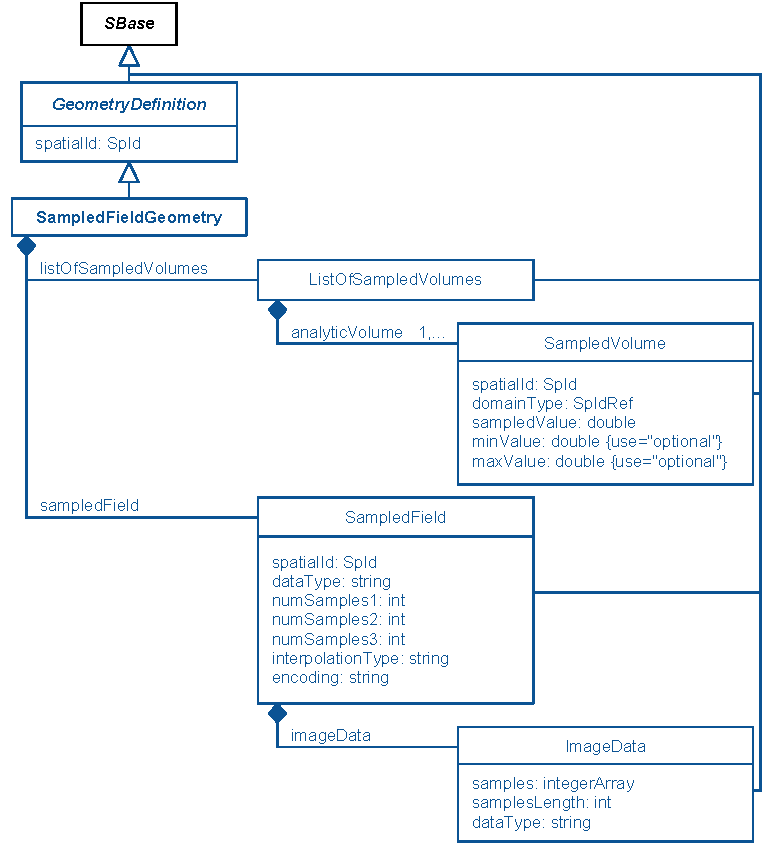
\includegraphics{figs/SampledFieldGeometry-uml}
  \caption{The definition of the \SampledFieldGeometry, \ListOfSampledVolumes, \SampledVolume, \SampledField, and \ImageData classes.}
  \label{SampledFieldGeometry-uml}
  \label{ListOfSampledVolumes-uml}
  \label{SampledVolume-uml}
  \label{SampledField-uml}
  \label{ImageData-uml}
\end{figure}



\subsection{The \class{SampledVolume} class}
\label{SampledVolume-class}
A \SampledVolume represents an interval of the sampled field that constitutes one or more contiguous regions. A \SampledVolume is defined for each volumetric (3-dimensional) \Domain in the \Geometry. It has the following attributes.

\subsubsection{The \token{\changed{id}} attribute}
The \token{\changed{id}} attribute identifies a \SampledVolume object. The attribute is of type \primtype{SpId} and is required when specifying a \SampledVolume.  It has no mathematical meaning.

\subsubsection{The \token{domainType} attribute}
The required \token{domainType} attribute is of type \primtype{SpIdRef}. It is the \changed{\primtype{SpId}} of the \DomainType that represents this class of anatomical features. If there are more than one contiguous regions, then more than one domain will be defined corresponding to each \SampledVolume.

\subsubsection{The \token{sampledValue} attribute}
The required \token{sampledValue} attribute is of type \primtype{double}. It represents the pixel value of a \SampledVolume.

\subsubsection{The \token{minValue} attribute}
The optional \token{minValue} attribute is of type \primtype{double}. It represents the minimum of the pixel value (\token{sampledValue}) range.

\subsubsection{The \token{maxValue} attribute}
The optional \token{maxValue} attribute is of type \primtype{double}. It represents the maximum of the pixel value (\token{sampledValue}) range.


\subsection{The \class{SampledField} class}
\label{SampledField-class}
A \SampledField defined in a \SampledFieldGeometry is a sampled scalar field such as an image or samples from a level set. Currently, the attributes of \SampledField represent the specification of an image dataset (the number of samples in x, y, z coordinates, data type of the image representation, etc.) and the ImageData element of the \SampledField specifies the actual image as integer sampled data.

\subsubsection{The \token{\changed{id}} attribute}
The \token{\changed{id}} attribute identifies a \SampledField. It is of type \primtype{SpId} and is a required attribute.  It has no mathematical meaning.

\subsubsection{The \token{numSamples1}, \token{numSamples2}, \token{numSamples3} attributes}
The \token{numSamples1}, \token{numSamples2}, and \token{numSamples3} attributes represent the number of samples in each of the coordinate components. (e.g. numX, numY, numZ) in an image dataset.  These attributes are of type \primtype{int} and are required to specify the \SampledField. The samples are assumed to be uniformly sampled.

\subsubsection{The \token{dataType} attribute}
This attribute represents the data type of each sample (e.g. int32). The attribute is of type \primtype{string} and is optional.

{\color{red} Lucian: \notice This attribute seems a bit arbitrary, and unhelpful unless there's a standard list of possible values here.  Is there one?  If not, I say we drop the attribute entirely.}


\subsubsection{The \token{interpolationType} attribute}
The \token{interpolationType} attribute is an optional attribute of type \primtype{string} and represents the interpolation type of the sampled data and is defined as "constant" for zeroth order, "linear" for first order, etc.

{\color{red} Lucian: \notice Again, the list of possible values here needs to be explicitly stated.  If it really can be any arbitrary order, switching this to a non-negative integer would make more sense.}

\subsubsection{The \token{encoding} attribute}
The \token{encoding} attribute is an optional attribute of type \primtype{string}. It is used to specify text encoding and compression.

{\color{red} Lucian: \notice Again, the list of possible values here needs to be explicitly stated, if it makes any difference to the model.  Unless you really want people to be able to put in 'standard zip' or 'rot13' as their encoding type.}


\subsection{The \class{ImageData} class}
\label{ImageData-class}
The ImageData element represents the actual image data of the image-based geometry as encoded samples defined by the encoding and the data type. The ImageData element has the following attributes.

\subsubsection{The \token{samples} attribute}
The \token{samples} attribute is of type \primtype{integerArray}, whose values represent the image pixel values. This attribute is required.

\subsubsection{The \token{samplesLength} attribute}
The \token{samplesLength} attribute is of type \primtype{int} and is required. It represents the array length of the \token{samples} attribute (number of values in the image data array).

\subsubsection{The \token{dataType} attribute}
The \token{dataType} attribute is of type \primtype{string} and is required. Presently, this attribute indicates if the image data is 'compressed' or 'uncompressed'.  {\color{red} Anu: \notice (This attribute and the \token{encoding} attribute of \SampledField have to be revisited.)}

{\color{red} Lucian: \notice I agree!}

\subsection{The \class{CSGeometry} class}
\label{CSGeometry-class}
\label{ListOfCSGObjects-class}
\CSGeometry (Constructed Solid Geometry) is a type of \GeometryDefinition that defines a combined, solid, volumetric object from a number of primitive solid volumes by the application of set operations such as union, intersection and difference and affine transformations such as rotation, scaling, translation, etc. The \CSGeometry element is defined by a \token{listOfCSGObjects} element that contains a collection of \CSGObjects. \fig{CSGeometry-uml} shows the definition of the \CSGeometry object.

\begin{figure}[ht]
  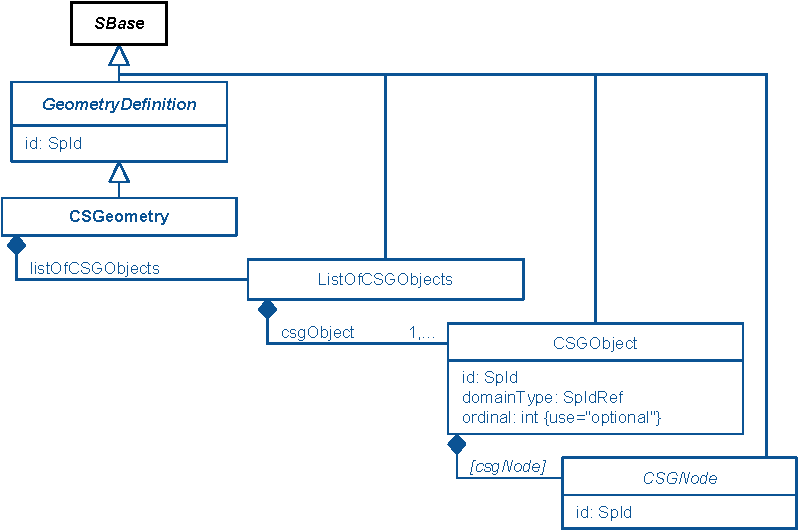
\includegraphics{figs/CSGeometry-uml}
  \caption{The definition of the \CSGeometry, \ListOfCSGObjects, and \CSGObject classes.}
  \label{CSGeometry-uml}
  \label{ListOfCSGObjects-uml}
  \label{CSGObject-uml}
\end{figure}



\subsection{The \class{CSGObject} class}
\label{CSGObject-class}
Each \CSGObject is a scene graph representing a particular geometric object using constructed solid geometry. A node in a tree (scene graph) is made up of \CSGPrimitives, \CSGSetOperators, and \CSGTransformations.  Note that the \CSGPrimitives are always leaves in this tree. The \CSGObject is analogous to an \AnalyticVolume element in the sense that it is a constructed geometry (from primitives) used to specify a volumetric (3-dimensional) domain. The \CSGObject element has three attributes : \token{\changed{id}}, \token{domain} and \token{ordinal}. The definition of the \CSGObject is completed by defining a \CSGNode which is the root of the \CSGObject scene graph.

\subsubsection{The \token{\changed{id}} attribute}
The \token{\changed{id}} attribute uniquely identifies the \CSGObject element. The attribute is required and is of type \primtype{SpId}. 

{\color{red} Lucian: \notice Does this element have mathematical meaning?}

\subsubsection{The \token{domain} attribute}
The \token{domain} attribute is of type \primtype{SpIdRef} and is a required attribute. It is a reference to the \token{\changed{id}} of the \Domain that this \CSGObject represents.

{\color{red} Lucian: \notice Am I correct in assuming that this information is redundant with the corresponding \Domain's interior points list?  Is this information necessarily redundant?  Is that OK?  I'm going to assume that the following is a reasonable restriction:}

All \InteriorPoints of the corresponding \Domain must be points inside the geometry this \CSGObject describes.

\subsubsection{The \token{ordinal} attribute}
The \token{ordinal} attribute of type \primtype{int} is an optional attribute. It is used to represent the order of the \CSGObject. The \token{ordinal} is useful while reconstructing the geometry in the specific software tool - it represents the order in which the \CSGObjects representing geometric domains have to be placed.

{\color{red} Lucian: \notice We should probably be as explicit here as we were with the similar \val{ordinal} attribute of the \AnalyticVolume class.  Can I assume that the same rules apply and copy the text here?  One oddness is that the \val{ordinal} attribute of the \AnalyticVolume class is optional, while here it is required.  If they do the same thing, we should probably either make them both optional, or both required.}


\subsubsection{The [\token{csgNode}] child}

The child [\token{csgNode}] element represents the geometry that is to be linked to the \token{domainType} of the \CSGObject.  Note that the child of the \CSGObject element is not called \val{csgNode} but rather takes the name of the derived class, decapitalized.  Thus, a \CSGObject may have a \token{csgPrimitive}, \token{csgPseudoPrimitive}, \token{csgSetOperator}, \token{csgTranslation}, \token{csgRotation}, \token{csgScale}, or \token{csgHomogeneousTransformation} child.


\subsection{The \class{CSGNode} class}
\label{CSGNode-class}
The operators and operands used to construct a constructed solid geometry are generalized as a \CSGNode, defined in \fig{CSGNode-uml} as an abstract base class. The classes that inherit from \CSGNode can be one of the following: \CSGSetOperator, \CSGTransformation (operators; itself another abstract base class), \CSGPrimitive, or \CSGPseudoPrimitive (operands). The \CSGNode has one attribute: \token{\changed{id}}. The \CSGObject contains a \CSGNode object which is the root of the \CSGObject scene graph (representing one constructed solid geometry domain).

\begin{figure}[ht]
  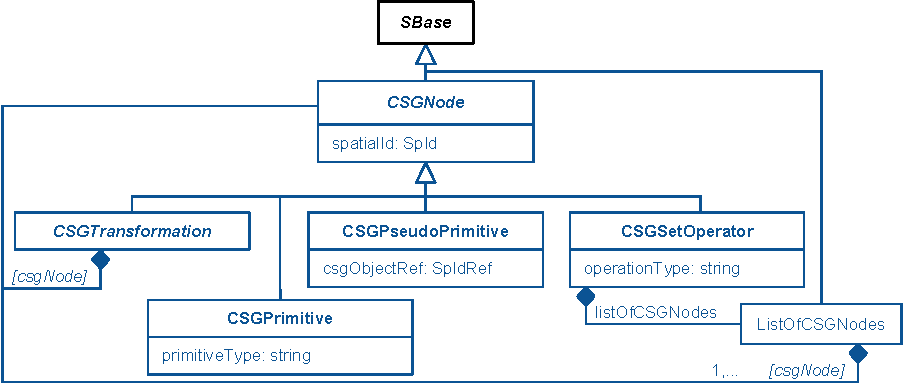
\includegraphics{figs/CSGNode-uml}
  \caption{The definition of the abstract base class \CSGNode, and its subclasses \CSGPrimitive, \CSGPseudoPrimitive, and \CSGSetOperator.  The abstract base class \CSGTransformation (also a subclass of \CSGNode) is defined in \sec{CSGTransformation-class}.}
  \label{CSGNode-uml}
  \label{CSGPrimitive-uml}
  \label{CSGPseudoPrimitive-uml}
  \label{CSGSetOperator-uml}
  \label{ListOfCSGNodes-uml}
\end{figure}

\subsubsection{The \token{\changed{id}} attribute}
The \token{\changed{id}} attribute uniquely identifies the \CSGNode element. The attribute is required and is of type \primtype{SpId}.

{\color{red} Lucian: \notice Do any of these classes have mathematical meaning?}


\subsection{The \class{CSGPrimitive} class}
\label{CSGPrimitive-class}
\CSGPrimitive element represents the primitive geometric shapes that can be represented by the \CSGeometry. Some of the primitive shapes that can be used are "sphere", "cylinder", "cube", "cone", etc. These shapes are defined with a predefined orientation and fitting within the unit cube (+/- 1 in x, y, and z). This element has one required attribute : \token{primitiveType} of type \primtype{string}.

\subsubsection{The \token{primitiveType} attribute}
The \token{primitiveType} attribute is a required attribute that is of type \primtype{string}. It represents one of the predefined primitive shapes.

{\color{red} Lucian: \notice This list absolutely needs to be included in the spec!}


\subsection{The \class{CSGPseudoPrimitive} class}
\label{CSGPseudoPrimitive-class}
\CSGPseudoPrimitive element is used to reference a pre-defined \CSGObject object while defining a \CSGObject (geometric domain). This allows the re-use of one constructed \CSGObject in another. It has one attribute of type \primtype{SpIdRef}.

\subsubsection{The \token{csgObjectRef} attribute}
The \token{csgObjectRef} attribute identifies a pre-defined \CSGObject in the \CSGeometry The attribute is required and is of type \primtype{SpId}.  A \CSGObject may not reference itself, nor its parent, nor its parent's parent, etc.


\subsection{The \class{CSGSetOperator} class}
\label{CSGSetOperator-class}
The \CSGSetOperator element represents the set operations (union, intersection, difference) that can be performed on a set of primitive geometric shapes (\CSGPrimitives) or on a set of \CSGNodes (a transformation or set operation on one or a set of \CSGPrimitives). This element has one attribute of type \primtype{string}. It also contains a required child \ListOfCSGNodes that represents the set of nodes on which the set operation is performed.

\subsubsection{The \token{operationType} attribute}
The \token{operationType} attribute is of type \primtype{SetOperation} and represents an operation that can be performed on a set of \CSGNodes. The possible values that the \token{operationType} attribute can take are \val{union}, \val{intersection} or \val{difference}.

{\color{red} Lucian: \notice 'union' and 'intersection' are unordered, but 'difference' is order-dependent, which is tricky to accomplish in the order-agnostic XML of SBML.  Either you have to say that order is important in this one case (something we've tried to avoid everywhere else), or we add an 'order' attribute somewhere, or we drop 'difference' as a possible set operator.  Also, according to wikipedia, the more common term is 'complement', with 'relative complement' and 'absolute complement' both meaning different things.}


\subsection{The \class{ListOfCSGNodes} class}
\label{ListOfCSGNodes-class}
The \ListOfCSGNodes must contain one or more \token{csgNode} children that are to be combined according to the set operation of the parent \CSGSetOperator.  While having a single child is legal, this is semantically equivalent to simply putting that child in the model instead of the \CSGSetOperator, and therefore has limited modeling benefit.  Note that the children of the \ListOfCSGNodes object are not called \token{csgNode} but rather take the name of the derived class, decapitalized.  Thus, they may be called \token{csgPrimitive}, \token{csgPseudoPrimitive}, \token{csgSetOperator}, \token{csgTranslation}, \token{csgRotation}, \token{csgScale}, or \token{csgHomogeneousTransformation}.


\subsection{The \class{CSGTransformation} class}
\label{CSGTransformation-class}
The \CSGTransformation represents a generalization for the type of transformation that can be performed on a primitive geometric shape (\CSGPrimitive) or on a \CSGNode (a transformation or set operation on one or a set of \CSGPrimitives). The types of possible transformations are 'rotation', 'translation', 'scaling', and 'homogeneous transformation', defined below. The \CSGTransformation element contains a \CSGNode element upon which the transformation is performed. It also has one attribute : transformationType of type \primtype{string}. 

\begin{figure}[ht]
  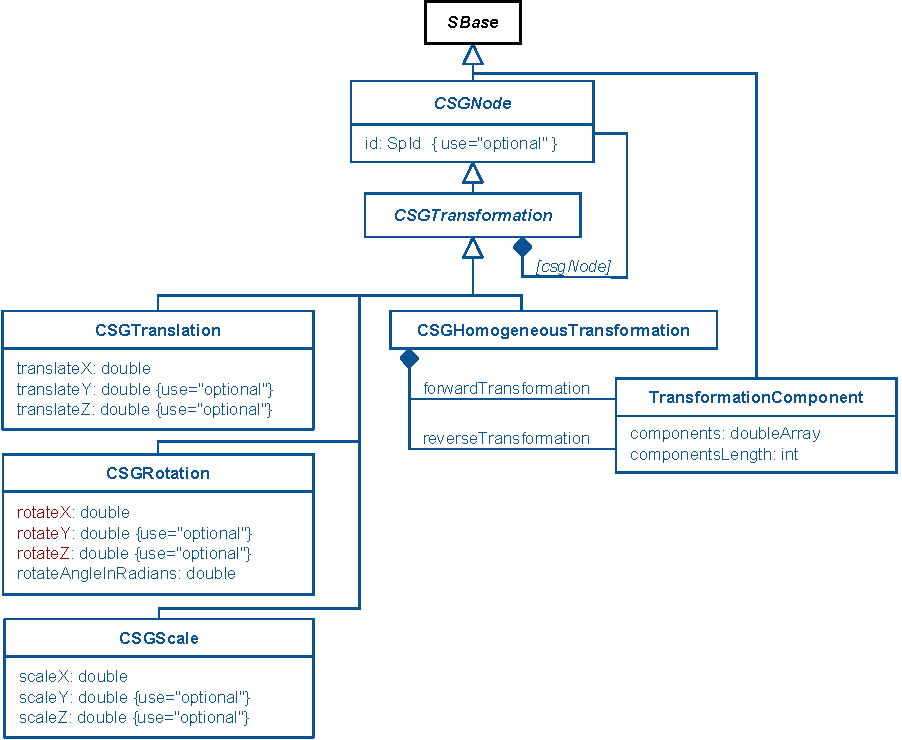
\includegraphics{figs/CSGTransformation-uml}
  \caption{The definition of the abstract base class \CSGTransformation, its subclasses, \CSGRotation, \CSGScale, and \CSGHomogeneousTransformation, and the \TransformationComponent class.}
  \label{CSGTransformation-uml}
  \label{CSGRotation-uml}
  \label{CSGScale-uml}
  \label{CSGHomogeneousTransformation-uml}
  \label{TransformationComponent-uml}
\end{figure}

\subsubsection{The transformationType attribute}
The transformationType attribute is of type \primtype{string} and is a required attribute. It represents the type of transformation ('rotation', 'translation', 'scaling', and 'homogeneous transformation').

{\color{red} Lucian: \notice This attribute didn't show up in the UML diagrams, and is redundant if the names of the elements are 'csgRotation', 'csgTranslation', etc.  I would strongly recommend the naming approach, as you've done this already, and I in fact already assumed it would be done this way.  If not... can we change it?  I dunno.}

\subsubsection{The \token{csgNode} child}

The child \token{csgNode} element represents the geometry that is to be transformed by the \CSGTransformation element.  Note that this child is not called \token{csgNode} but rather takes the name of the derived class, decapitalized.  Thus, it may be called \token{csgPrimitive}, \token{csgPseudoPrimitive}, \token{csgSetOperator}, \token{csgTranslation}, \token{csgRotation}, \token{csgScale}, or \token{csgHomogeneousTransformation}.


\subsection{The \class{CSGTranslation} class}
\label{CSGTranslation-class}
The \CSGTranslation element represents a translation transformation on a \CSGNode (a transformation or set operation on one or a set of \CSGPrimitives) or a \CSGPrimitive along the axes defined in the \Geometry. This element has 3 attributes:

\subsubsection{The \token{translateX} attribute}
The \token{translateX} attribute is of type \primtype{double}. It represents the translation of the \CSGNode along the x-axis (the \CoordinateComponent with the \token{\changed{type}} of \val{cartesianX}).

\subsubsection{The \token{translateY} attribute}
The \token{translateY} attribute is of type \primtype{double}. It represents the translation of the \CSGNode along the y-axis (the \CoordinateComponent with the \token{\changed{type}} of \val{cartesianY}).

\subsubsection{The \token{translateZ} attribute}
The \token{translateZ} attribute is of type \primtype{double}. It represents the translation of the \CSGNode along the z-axis (the \CoordinateComponent with the \token{\changed{type}} of \val{cartesianZ}).

{\color{red} Lucian: \notice I still think it's awkward to have attributes here that correspond to attribute *values* somewhere else, but it's at least not incorrect, like it was before we stripped everything but the cartesian coordinate system.  Not sure what a good fix would be, though.}

\subsection{The \class{CSGRotation} class}
\label{CSGRotation-class}
The \CSGRotation element represents a rotation transformation on a \CSGNode (a transformation or set operation on one or a set of \CSGPrimitives) or a \CSGPrimitive about the axes defined in the \Geometry. This element has 4 attributes:

\subsubsection{The \token{rotateX} attribute}
The \token{rotateX} attribute is of type \primtype{double}. It represents the rotation of the \CSGNode along the x-axis (the \CoordinateComponent with the \token{\changed{type}} of \val{cartesianX}).

{\color{red} Lucian: \notice I don't know what 'the rotation' means, since there's already an angle attribute.  Are we talking relative rotation of that angle on this axis?  I think we need more semantics here.}

\subsubsection{The \token{rotateY} attribute}
The \token{rotateY} attribute is of type \primtype{double}. It represents the rotation of the \CSGNode along the y-axis (the \CoordinateComponent with the \token{\changed{type}} of \val{cartesianY}).

\subsubsection{The \token{rotateZ} attribute}
The \token{rotateZ} attribute is of type \primtype{double}. It represents the rotation of the \CSGNode along the z-axis (the \CoordinateComponent with the \token{\changed{type}} of \val{cartesianZ}).


\subsubsection{The \token{rotationAngleInRadians} attribute}
The \token{rotationAngleInRadians} attribute is of type \primtype{double}. It represents the rotation angle of the \CSGNode, in radians, along the defined axis.


\subsection{The \class{CSGScale} class}
\label{CSGScale-class}
The \CSGScale element represents a scale transformation on a \CSGNode (a transformation or set operation on one or a set of \CSGPrimitives) or a \CSGPrimitive along the axes defined in the \Geometry. This element has 3 attributes:

{\color{red} Lucian: \notice Does it make a difference if the object is scaled and remains centered where it was, or leaves its corner at the origin?  If so, the version used should be explicitly stated here, I think.}

\subsubsection{The \token{scaleX} attribute}
The \token{scaleX} attribute is of type \primtype{double}. It represents the amount of scaling of the \CSGNode along the x-axis (the \CoordinateComponent with the \token{\changed{type}} of \val{cartesianX}).

\subsubsection{The \token{scaleY} attribute}
The \token{scaleY} attribute is of type \primtype{double}. It represents the amount of scaling of the \CSGNode along the y-axis (the \CoordinateComponent with the \token{\changed{type}} of \val{cartesianY}).

\subsubsection{The \token{scaleZ} attribute}
The \token{scaleZ} attribute is of type \primtype{double}. It represents the amount of scaling of the \CSGNode along the z-axis (the \CoordinateComponent with the \token{\changed{type}} of \val{cartesianZ}).

\subsection{The \class{CSGHomogeneousTransformation} class}
\label{CSGHomogeneousTransformation-class}
The \CSGHomogeneousTransformation element represents a homogeneous transformation on a \CSGNode: a transformation or set operation on one or more \CSGPrimitives. This element contains two TransformationComponent elements : a \token{forwardTransformation} and a \token{reverseTransformation}, both of type \TransformationComponent.

{\color{red} Lucian: \notice The difference between the forward and reverse transformations needs to be explained here, as well as why you need both.}


\subsection{The \class{TransformationComponent} class}
\label{TransformationComponent-class}
The \TransformationComponent element represents an affine transformation that can be applied to a \CSGNode. This element has the following two attributes:

\subsubsection{The \token{components} attribute}
The \token{components} attribute is of type \primtype{doubleArray}, whose values represent the affine transformation. This attribute is required.

\subsubsection{The \token{componentsLength} attribute}
The \token{componentsLength} attribute is of type \primtype{int} and is required. It represents the array length of the \token{components} attribute (number of values in the \token{components} array).


\subsection{The \class{ParametricGeometry} class}
\label{ParametricGeometry-class}
\label{ListOfSpatialPoints-class}
\label{ListOfParametricObjects-class}
\ParametricGeometry is a type of \GeometryDefinition that parametrically defines geometric strucutures/domains. The \ParametricGeometry element is defined with a \token{listOfObjects} that is a collection of \ParametricObjects and a \token{listOfSpatialPoints} that is a collection of \SpatialPoints. \fig{ParametricGeometry-uml} shows the definition of the \ParametricGeometry object.

\begin{figure}[ht]
  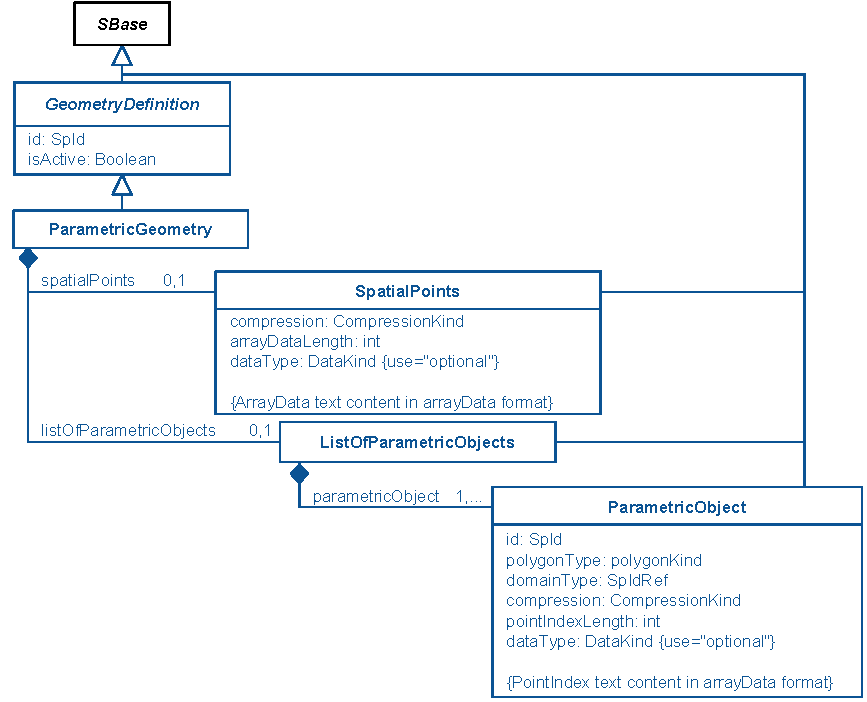
\includegraphics{figs/ParametricGeometry-uml}
  \caption{The definition of the \ParametricGeometry, \ListOfSpatialPoints, \SpatialPoint, \ListOfParametricObjects, \ParametricObject, and \PolygonObject classes.}
  \label{ParametricGeometry-uml}
  \label{ListOfSpatialPoints-uml}
  \label{SpatialPoint-uml}
  \label{ListOfParametricObjects-uml}
  \label{ParametricObject-uml}
  \label{PolygonObject-uml}
\end{figure}


\subsection{The \class{ParametricObject} class}
\label{ParametricObject-class}
The \ParametricObject element represents a parametric geometry object. 

\subsubsection{The \token{\changed{id}} attribute}
The \token{\changed{id}} attribute is a required attribute of type \primtype{SpId}. It uniquely identifies the \ParametricObject element.

{\color{red} Lucian: \notice Does this element have mathematical meaning?}

\subsubsection{The \token{polygonType} attribute}
The \token{polygonType} attribute is of type \primtype{string} and is a required attribute. It represents the type of polygon that describes the \ParametricObject.

{\color{red} Lucian: \notice What options are there for this attribute?}

\subsubsection{The \token{domain} attribute}
The \token{domain} attribute is of type \primtype{SpIdRef} and is a required attribute. It is a reference to the \token{\changed{id}} of the domain that this \ParametricObject represents.

{\color{red} Lucian: \notice As above:  Am I correct in assuming that this information is redundant with the corresponding \Domain's interior points list?  Is this information necessarily redundant?  Is that OK?  I'm going to assume that the following is a reasonable restriction:}

All \InteriorPoints of the corresponding \Domain must be points inside the geometry this \ParametricObject describes.


\subsection{The \class{PolygonObject} class}
\label{PolygonObject-class}
The polygonObject represents an ordered list of indices that refer to elements in the SpatialPoints array and are interpreted by considering the \token{polygonType} attribute of the \ParametricObject.  For reference, we could consider using the VTK polydata convensions for shapes and vertex orderings.

{\color{red} Lucian: \notice Wait, 'consider'?  Are there other options?  If so, how would the modeler know that a different conversion was being followed?  Or does it not matter?}


\subsubsection{The \token{pointIndex} attribute}
The \token{pointIndex} attribute is an array of integers holding the indices of the points in the SpatialPoints array.


\subsection{The \class{SpatialPoint} class}
\label{SpatialPoint-class}
The \SpatialPoint element represents a point used as a vertex in the \ParametricGeometry.

\subsubsection{The \token{\changed{id}} attribute}
The \token{\changed{id}} element uniquely identifies a SpatialPoint element. It is a required attribute and is of type \primtype{SpId}.

{\color{red} Lucian: \notice Does this element have mathematical meaning?}

\subsubsection{The \token{coord1}, \token{coord2}, and \token{coord3} attributes}
The \token{coord1}, \token{coord2}, \token{coord3} attributes are of type \primtype{double}. They represent the 3-dimensional coordinate of the SpatialPoint. Depending on the dimension of the \Geometry, one, two or all the three attributes are required. 

\subsubsection{The \token{domain} attribute}
The \token{domain} attribute is of type \primtype{SpIdRef} and is a required attribute. It is a reference to the \token{\changed{id}} of the domain which contains this SpatialPoint.

{\color{red} Lucian: \notice And once more:}

All \InteriorPoints of the corresponding \Domain must be points inside the geometry this \SpatialPoint describes.

